\documentclass[11pt]{report}
% this template is originally from Roy Dong's ECE 515.
% Editted by Dawei Sun
%%%%%%%%%%%%%%%%%%%%%%%%%%%%%%%%%%%%%%%%%%%%%%%%%%%%%%%%%%%%%%%%%%
% Set the margins of our document.
\usepackage[margin = 1 in]{geometry}

%%%%%%%%%%%%%%%%%%%%%%%%%%%%%%%%%%%%%%%%%%%%%%%%%%%%%%%%%%%%%%%%%%
% Import commands for custom header.
\usepackage{fancyhdr}
\pagestyle{fancy}

%%%%%%%%%%%%%%%%%%%%%%%%%%%%%%%%%%%%%%%%%%%%%%%%%%%%%%%%%%%%%%%%%%
% Allow ourselves to do equations!
\usepackage{amsmath,amssymb,amsthm}
\usepackage{bm}
\usepackage{upgreek}

%%%%%%%%%%%%%%%%%%%%%%%%%%%%%%%%%%%%%%%%%%%%%%%%%%%%%%%%%%%%%%%%%%
% Nicer formatting for enumerate commands.
\usepackage[shortlabels]{enumitem}

%%%%%%%%%%%%%%%%%%%%%%%%%%%%%%%%%%%%%%%%%%%%%%%%%%%%%%%%%%%%%%%%%%
% Colored text and include images.
\usepackage{color}
\usepackage{graphicx}
\usepackage{mathtools}
\usepackage{bbm}

\usepackage{hyperref}
\hypersetup{
    colorlinks=true,
    linkcolor=blue,
    filecolor=magenta,
    urlcolor=cyan,
}

\urlstyle{same}

%%%%%%%%%%%%%%%%%%%%%%%%%%%%%%%%%%%%%%%%%%%%%%%%%%%%%%%%%%%%%%%%%%
% Some custom macros to make life easier.
\DeclarePairedDelimiter\ceil{\lceil}{\rceil}
\DeclarePairedDelimiter\floor{\lfloor}{\rfloor}
\newcommand{\mc}{\mathcal}
\newcommand{\mb}{\mathbb}
\newcommand{\vect}[1]{\boldsymbol{\mathbf{#1}}}
\newcommand{\T}{\intercal}
\newcommand{\E}[1]{\mathbb{E}\left[#1\right]}
\newcommand{\condi}[2]{#1 \ | \ #2}
%%%%%%%%%%%%%%%%%%%%%%%%%%%%%%%%%%%%%%%%%%%%%%%%%%%%%%%%%%%%%%%%%%
%%%%%%%%%%%%%%%%%%%%%%%%%%%%%%%%%%%%%%%%%%%%%%%%%%%%%%%%%%%%%%%%%%
%%%%%%%%%%%%%%%%%%%%%%%%%%%%%%%%%%%%%%%%%%%%%%%%%%%%%%%%%%%%%%%%%%

\lhead{ECE 543 - Spring 2020 at University of Illinois at Urbana-Champaign}
\rhead{\textcolor{red}{HOMEWORK2}}
\lfoot{Submitted by: Dawei Sun (\textcolor{red}{\textit{daweis2}})}

%%%%%%%%%%%%%%%%%%%%%%%%%%%%%%%%%%%%%%%%%%%%%%%%%%%%%%%%%%%%%%%%%%
%%%%%%%%%%%%%%%%%%%%%%%%%%%%%%%%%%%%%%%%%%%%%%%%%%%%%%%%%%%%%%%%%%
%%%%%%%%%%%%%%%%%%%%%%%%%%%%%%%%%%%%%%%%%%%%%%%%%%%%%%%%%%%%%%%%%%

\begin{document}

%%%%%%%%%%%%%%%%%%%%%%%%%%%%%%%%%%%%%%%%%%%%%%%%%%%%%%%%%%%%%%%%%%
%%%%%%%%%%%%%%%%%%%%%%%%%%%%%%%%%%%%%%%%%%%%%%%%%%%%%%%%%%%%%%%%%%
%%%%%%%%%%%%%%%%%%%%%%%%%%%%%%%%%%%%%%%%%%%%%%%%%%%%%%%%%%%%%%%%%%

%\pagebreak
\section*{Problem 1}
\subsection*{Solution}
\begin{enumerate}[(a)]
\item Let $t = \sqrt{1+x}$. Since $x \geq 0$, we have $t \geq 1$. Let $h(t) = 2\log(t) - t$, then we have to prove that $h(t) \leq 0$ holds for all $t \geq 1$. Since $h'(t) = \frac{2}{t}-1$, we have $h(t) \leq h(2) < 0$.
\item Let $h(m) = \frac{\log(m)}{m}, m \geq 1$. We have $h'(m) = \frac{1-\log(m)}{m^2}$. Thus, $h(m)$ is decreasing when $m \geq e$.

If $n=1$, then $m < \log(m)$ $\implies$ $m<0$. (Acutually, the inequality on left hand is not possible for all $m$, and thus it can imply any statement.) Similarly, it is trivial if $m=1$. For the cases where $n \geq 2$ and $m \geq 2$, we proceed by contradiction. Suppose that $m \geq 2n\log(n) > e$. Since $\frac{m}{\log(m)}$ is increasing when $m \geq e$ and $n \geq 2\log(n)$ (conclusion of (a)), we have $\frac{m}{\log(m)} \geq \frac{2n\log(n)}{\log(2n\log(n))} \geq \frac{2n\log(n)}{\log(n^2)} = n$. Thus $m < n\log(m)$ $\implies$ $m < 2n\log(n)$.
\end{enumerate}
\section*{Problem 2}
\subsection*{Solution}
The Lagrangian of this problem is $$L(w, b, \xi, \mu, \lambda) = \frac{1}{2} ||w||^2 + C\sum_{i=1}^{n} \xi_i + \sum_{i=1}^{n} \mu_i(1-\xi_i-y_i(w^\T x_i+b)) - \sum_{i=1}^{n} \lambda_i \xi_i,~\mu_i \geq 0~and~\lambda_i \geq 0.$$
Let the gradient of $L$ w.r.t $w$, $b$ and $\xi$ be $0$. We have
$$\nabla_w L = w - \sum_{i=1}^{n} \mu_i y_i x_i = 0,$$
$$\nabla_b L = \sum_{i=1}^{n} \mu_i y_i = 0,$$
$$\nabla_{\xi_i} L = C - \lambda_i - \mu_i = 0,~\forall i.$$
Since $C = \lambda_i - \mu_i = 0,~\forall i$ and $\lambda_i \geq 0$, we have $\mu_i \leq C$.
By substituting $w = \sum_{i=1}^{n} \mu_i y_i x_i$, we have $D(\mu, \lambda) = \sum_{i=1}^{n} \mu_i - \frac{1}{2}\sum_{i=1}^{n}\sum_{j=1}^{n}\mu_i\mu_jy_iy_j(x_i^\T x_j)$, and $\lambda$ doesn't appear in the objective function and constraints. Thus, the dual problem is of the same form as the soft-margin version with additional constraints that $\mu_i \leq C,~\forall i$.

\section*{Problem 3}
\subsection*{Solution}
Let $L_t(\alpha) = \sum_{i=1}^{n} \exp\left(-\sum_{s=1}^{t-1} \alpha_s y_i h_s(x_i) - \alpha y_i h_t(x_i)\right)$. Then, $\alpha_t = \arg\min L_t(\alpha)$. Suppose that $h_{t+1} = h_t$. Then, $L_{t+1}(\alpha) = L_t(\alpha +\alpha_t)$. Thus, $\alpha_{t+1} = 0 = \arg\min L_{t+1}(\alpha)$. However, since $\epsilon_t < \frac{1}{2}$, $\alpha_{t+1} = \frac{1}{2} \ln \frac{1-\epsilon_{t+1}}{\epsilon_{t+1}} > 0$. Thus, by contradiction, $h_{t+1} \neq h_t$.
\section*{Problem 4}
\subsection*{Solution}
\begin{enumerate}[(a)]
\item $91\%$.
\item As shown in Fig.~\ref{fig:adaboost}, test accuracy improves as number of learners increases.
\begin{figure}
  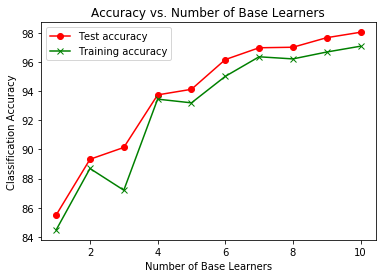
\includegraphics{adaboost.png}
  \caption{Results of AdaBoost.}
  \label{fig:adaboost}
\end{figure}
\end{enumerate}
\section*{Problem 4}
\subsection*{Solution}
\begin{enumerate}[(a)]
\item Accuracies are $50\%, 50\%, 52\%, 69\%, 97\%, 98\%$ respectively.
\item Linear kernel: $98\%$. Poly kernel: $99\%$. RBF kernel: $100\%$. Sigmoid kernel: $81\%$.
\end{enumerate}
\end{document}
